\documentclass[12pt,a4paper]{article}
%-------------------------------------------
%---Packages--------------------------------
%-------------------------------------------
\usepackage[utf8]{inputenc}
%\usepackage[T1]{fontenc}
%\usepackage{txfonts}
\usepackage{amsmath}
\usepackage{amsthm}
\usepackage{amsfonts}
\usepackage{array}
\usepackage{amssymb}
\usepackage{blindtext}
\usepackage{caption}
\usepackage{color}
\usepackage{csquotes}	    %
\usepackage{enumitem}	    %pour mieux bosser avec les listes. ajoute option label
\usepackage[yyyymmdd]{datetime}        %pour définir date custom
\usepackage{etaremune}
\usepackage{environ}
\usepackage{fancybox}
\usepackage{fancyhdr} 	    % Custom headers and footers
\usepackage{fancyref}
%\usepackage{float}
\usepackage{floatrow}       %float and floatrow can't be together...
\usepackage{gensymb}
\usepackage{graphicx}
\usepackage[colorlinks=true, linkcolor=purple, citecolor=cyan]{hyperref}
\usepackage{footnotebackref}
\usepackage{lipsum}
\usepackage{mathtools}
\usepackage{multicol}	    %gérer plusieurs colonnes
\usepackage{setspace}
\usepackage{subcaption}
\usepackage{todonotes}	    %Bonne gestion des TODOs
%TODO commenté pour tester l'utilité... à voir% \usepackage[tc]{titlepic}      %Permet de mettre une image en page de garde
\usepackage{tikz}	    % Pour outil de dessin puissant
\usepackage{ulem}	    %underline sur plusieurs lignes (avec \uline{})
\usepackage{vmargin} 	    %gestion des marges, avec dans l'ordre : gauche, haut, droit, bas, en-tête, entre en-tête et texte, bas de page, hauteur entre bas de page et texte
\usepackage{wrapfig}
\usepackage{xcolor}
\usepackage{xparse}                    %Pour utiliser NewDocumentCommand et des arguments 'mmooo'
%\usepackage{fullpage} 	    %supprime toutes les marges allouées aux notes, aussi en haut et en bas

%\ExplSyntaxOn
\pagestyle{fancyplain}	    %Makes all pages in the document conform to the custom headers and footers

%-------------------------------------------
%---Document Commands-----------------------
%---------------------------{----------------
\NewDocumentCommand{\framecolorbox}{oommm}
 {% #1 = width (optional)
  % #2 = inner alignment (optional)
  % #3 = frame color
  % #4 = background color
  % #5 = text
  \IfValueTF{#1}%
   {\IfValueTF{#2}%
    {\fcolorbox{#3}{#4}{\makebox[#1][#2]{#5}}}%
    {\fcolorbox{#3}{#4}{\makebox[#1]{#5}}}%
   }%
   {\fcolorbox{#3}{#4}{#5}}%
 }%
%------------------------------------------------
%------------------ENGLISH----------------------
%----------------------------------------------

\NewDocumentCommand{\epflTitle}{mO{Olivier Cloux}O{\today}O{Notes de Cours en}D<>{../../Common}}%Arguments : Matière, Auteur, Date, Titre du doc
{
\begin{titlepage}
    \vspace*{\fill}
    \begin{center}
        \normalfont \normalsize
        \textsc{Ecole Polytechnique Fédérale de Lausanne} \\ [25pt] % Your university, school and/or department name(s)
        \textsc{#4} %Titre du doc
        \\ [0.4 pt]
        \horrule{0.5pt} \\[0.4cm] % Thin top horizontal rule
        \huge #1 \\ % Matière
        \horrule{2pt} \\[0.5cm] % Thick bottom horizontal rule
        
\includegraphics[width=8cm]{#5/EPFL_logo}
        ~\\[0.5 cm]
        \small\textsc{#2}\\[0.4cm]
        \small\textsc{#3}\\
        ~\\
        ~\\
        
\includegraphics[scale=0.5]{#5/creativeCommons}
    \end{center}
    \vspace*{\fill}
\end{titlepage}
}


%-------------------------------------------
%-------------MATH NEW COMMANDS-------------
%-------------------------------------------
\newcommand{\somme}[2]{\ensuremath{\sum\limits_{#2}^{#1}}}
\newcommand{\produit}[2]{\ensuremath{\prod\limits_{#2}^{#1}}}
\newcommand{\limite}{\lim\limits_}
\newcommand{\llimite}[3]{\limite{\substack{#1 \\ #2}}\left(#3\right)}	%limites à deux condiitons
\newcommand{\et}{\mbox{ et }}
\newcommand{\deriv}[1]{\ensuremath{\, \mathrm d #1}}	%sigle dx, dt,dy... des dérivées/intégrales
%\newcommand{\fx}{\ensuremath{f'(\textbf{x}_0 + h}}
\newcommand{\ninf}{\ensuremath{n \to \infty}}	       %pour les limites : n tend vers l'infini
\newcommand{\xinf}{\ensuremath{x \to \infty}}	       %pour les limites : x tend vers l'infini
\newcommand{\infint}{\ensuremath{\int_{-\infty}^{\infty}}}
\newcommand{\xo}{\ensuremath{x \to 0}}									%x to 0
\newcommand{\no}{\ensuremath{n \to 0}}									%n zéro
\newcommand{\xx}{\ensuremath{x \to x}}									%x to x
\newcommand{\Xo}{\ensuremath{x_0}}										%x zéro
\newcommand{\X}{\ensuremath{\mathbf{X}} }
\newcommand{\A}{\ensuremath{\mathbf{A}} }
\newcommand{\R}{\ensuremath{\mathbb{R}} }								%ensemble de R
\newcommand{\rn}{\ensuremath{\mathbb{R}^n} } 							%ensemble de R de taille n
\newcommand{\Rm}{\ensuremath{\mathbb{R}^m} }  							%ensemble de R de taille m
\newcommand{\C}{\ensuremath{\mathbb{C}} }
\newcommand{\N}{\ensuremath{\mathbb{N}} }
\newcommand{\Z}{\ensuremath{\mathbb{Z}} }
\newcommand{\Q}{\ensuremath{\mathbb{Q}} }
\newcommand{\rtor}{\ensuremath{\R \to \R} }
\newcommand{\pour}{\mbox{ pour }}
\newcommand{\coss}[1]{\ensuremath{\cos\(#1\)}}						%cosinus avec des parenthèses de bonne taille (genre frac)
\newcommand{\sinn}[1]{\ensuremath{\sin\(#1\)}}					%sinus avec des parentèses de bonne taille (genre frac)
\newcommand{\txtfrac}[2]{\ensuremath{\frac{\text{#1}}{\text{#2}}}}		%Fractions composées de texte
\newcommand{\evalfrac}[3]{\ensuremath{\left.\frac{#1}{#2}\right|_{#3}}}
\renewcommand{\(}{\left(}												%Parenthèse gauche de taille adaptive
\renewcommand{\)}{\right)}
\newcommand{\longeq}{=\joinrel=}												%Parenthèse droite de taille adaptive


%-------------------------------------------------------
%------------------MISC NEW COMMANDS--------------------
%-------------------------------------------------------
\newcommand{\degre}{\ensuremath{^\circ}}
%\newdateformat{\eudate}{\THEYEAR-\twodigit{\THEMONTH}-\twodigit{\THEDAY}}



%-------------------------------------------------------
%------------------TEXT NEW COMMANDS--------------------
%-------------------------------------------------------
\newcommand{\ts}{\textsuperscript}
\newcommand{\evid}[1]{\textbf{\uline{#1}}}        %mise en évidence (gras + souligné)



%\newcommand{\Exemple}{\underline{Exemple}}
\newcommand{\Theoreme}{\underline{Théorème}}
\newcommand{\Remarque}{\underline{Remarque}}
\newcommand{\Definition}{\underline{Définition} }
\newcommand{\skinf}{\sum^{\infty}_{k=0}}
\newcommand{\combi}[2]{\ensuremath{\begin{pmatrix} #1 \\ #2 \end{pmatrix}}}	%combinaison parmi 1 de 2
\newcommand{\intx}[3]{\ensuremath{\int_{#1}^{#2} #3 \deriv{x}}}				%intégrale dx
\newcommand{\intt}[3]{\ensuremath{\int_{#1}^{#2} #3 \deriv{t}}}				%intégrale dy
\newcommand{\misenforme}{\begin{center} Mis en forme jusqu'ici\\ \line(1,0){400}\\ normalement juste, mais à améliorer depuis ici\end{center}}	%raccourci pour mise en forme
\newcommand*\circled[1]{\tikz[baseline=(char.base)]{
            \node[shape=circle,draw,inner sep=1pt] (char) {#1};}}			%pour entourer un chiffre
\newcommand{\horrule}[1]{\rule{\linewidth}{#1}} 				% Create horizontal rule command with 1 argument of height

\theoremstyle{definition}
\newtheorem{exemp}{Exemple}
\newtheorem{examp}{Example}


%-------------------------------------------
%---Environments----------------------------
%-------------------------------------------
\NewEnviron{boite}[1][0.9]{%
	\begin{center}
		\framecolorbox{red}{white}{%
			\begin{minipage}{#1\textwidth}
 	 			\BODY
			\end{minipage}
		}
	\end{center}
}
\NewEnviron{blackbox}[1][0.9]{%
	\begin{center}
		\framecolorbox{black}{white}{%
			\begin{minipage}{#1\textwidth}
 	 			\BODY
			\end{minipage}
		}
	\end{center}
}
\NewEnviron{exemple}[1][0.8]{%
    \begin{center}
        \framecolorbox{white}{gray!20}{%
            \begin{minipage}{#1\textwidth}
                \begin{exemp}
                    \BODY
                \end{exemp}
            \end{minipage}
        }
    \end{center}
}
\NewEnviron{suiteExemple}[1][0.8]{%
    \begin{center}
        \framecolorbox{white}{gray!20}{%
            \begin{minipage}{#1\textwidth}
                \BODY
            \end{minipage}
        }
    \end{center}
}
\NewEnviron{colExemple}[1][0.8]{%
    \begin{center}
        \framecolorbox{white}{gray!20}{%
            \begin{minipage}{#1\columnwidth}
                \begin{exemp}
                    \BODY
                \end{exemp}
            \end{minipage}
        }
    \end{center}
}
\NewEnviron{example}[1][0.8]{%
    \begin{center}
        \framecolorbox{white}{gray!20}{%
            \begin{minipage}{#1\textwidth}
                \begin{examp}
                    \BODY
                \end{examp}
            \end{minipage}
	}
    \end{center}
}
\NewEnviron{systeq}[1][l]{
			\begin{center}
				$\left\{\begin{array}{#1}
					\BODY
				\end{array}\right.$
			\end{center}
 }





%-------------------------------------------
%---General settings-----------------------
%-------------------------------------------
\renewcommand{\headrulewidth}{1pt}										%ligne au haut de chaque page
\renewcommand{\footrulewidth}{1pt}										%ligne au pied de chaque page
\setstretch{1.6}
\author{Olivier Cloux}

\usepackage[tc]{titlepic}
\usepackage{graphicx}
\usepackage{blindtext}
%\usepackage[a4paper]{geometry}
%\setcounter{section}{-1}
\date{Printemps 2015}
\title{	
\normalfont \normalsize 
\textsc{Ecole Polytechnique Fédérale de Lausanne} \\ [25pt] % Your university, school and/or department name(s)
\textsc{Note de cours en }\\ [0pt] %Name of the course
\horrule{0.5pt} \\[0.4cm] % Thin top horizontal rule
\huge Electronique I\\ % The assignment title<
\horrule{2pt} \\[0.5cm] % Thick bottom horizontal rule

\includegraphics[width=8cm]{images/EPFL_logo}
}
\renewcommand{\contentsname}{Table des Matières}
\begin{document}
\setstretch{1}
\maketitle
\newpage
\tableofcontents
\setstretch{1.2}
\section{Week 2}
Rappels de base : 
\begin{itemize}
	\item I = courant = charges en déplacement (dynamique)
	\item U = tension = charges disponibles (statique). Se mesure entre deux bornes (par ex. d'une résistance).
\end{itemize}
Un signal qui est positif puis négatif périodiquement est alternatif. Si on retrouve sa configuration plus loin, il est périodique. On verra en analyse que tout signal "sinusoidal" (même carré, triangulaire,...) peut se décomposer en une infinité de sinus (une série de Fourrier). Les valeurs à crête représentent aussi bien le sommet que le creux du signal.  Une source indépendante sera toujours représentée par un rond. 
\begin{boite}
	\evid{Conventions :}\\
	\uline{Signaux continus} : Majuscules : U,V,I,...\\
	\uline{Signaux variables} : minuscules : $u(t), i(t), \uline{u}, \uline{v}, \uline{i},...$. Les soulignés représentent des complexes\\
	\uline{Courant d'électrons inverse au sens du courant}
	
	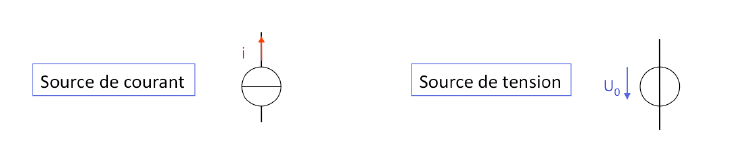
\includegraphics[scale=0.5]{images/conventions_dessins}
\end{boite}
Le courant est tout a fait relatif par rapport à la "terre", ou "masse". On sera à un potentiel par rapport à une référence. Être en altitude et avoir tous les appareils à 15M voltes n'est pas intéressant à savoir. Si on est a 5V au dessus de la masse, alors on comptera 5 voltes.\\
Equipotentielle : chaque fil a une résistance. On parlera de circuit equipotentiel.

Avec des résistances en parallèles, la résistance totale est toujours plus petite que la plus petite des deux.

\section{Semaine 3 : Rappels sur les composants}
\begin{figure}[!h]
	\centering
	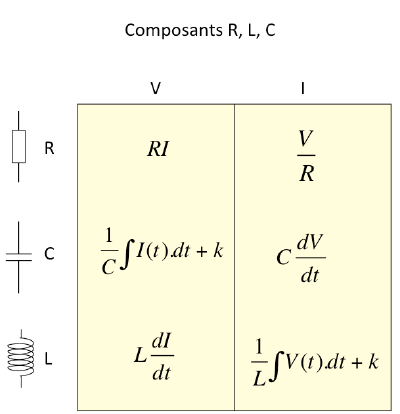
\includegraphics[scale=0.5]{images/resume_composants}
\end{figure}
\subsection{Résistance}
\subsection{Condensateur}
\subsection{Inductance}
Pas de lien avec l'hydraulique. 

\subsection{Des Théorèmes}
Quelques définitions : 
\begin{itemize}
	\item 	Un réseaux est composé de multitudes de segments
	\item 	Une branche est composée d'une série de segments.
	\item 	Un n\oe ud est un point du réseau relié au moins à 2 branches.
	\item 	Une maille est un parcours fermé, constitué de branches, ne passant qu'une seule fois par un n\oe ud donné 
\end{itemize}
\subsubsection{Kirchhoff}
Deux lois essentielles :
\begin{align}
	\text{Dans un cycle : } \sum U_i = 0\\
	\text{Dans un n\oe ud : } \sum I_{sortants} - \sum I_{entrant} = 0
\end{align}
Rien ne se perd, rien ne se crée,...\\
Un n\oe ud intéressant est composé d'au moins 3 segments. Sinon le rentrant est le même que le rentrant...
\subsubsection{Théorème de Millman}
\begin{wrapfigure}{r}{5.5cm}
\centering
\captionsetup{justification=centering}
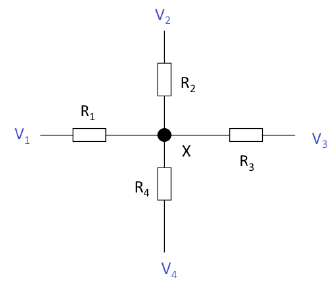
\includegraphics[scale=0.7]{images/millman}
\caption{Un exemple de n\oe ud}
\end{wrapfigure}
Le théorème de Millman est issu des lois de kirchoff. Il permet de calculer une tension d'un n\oe ud quelconque en fonction de son voisinage. On peut choisir le sens des courants et tensions, puis s'y tenir. Ça a du sens, car nous obtiendrons des résultats négatifs pour les "mauvais sens"
\begin{equation}
\tag{Millman}
V_x = \frac{\somme{i=1}{N} \frac{V_i}{R_i}}{\somme{i=1}{N}\frac{1}{R_i}}
\end{equation}

\subsection{Simplifications}
\subsubsection{Résistances}
\evid{Série}. Prouver que deux résistances en série se simplifient par leur addition. Lois des mailles sur un coin du circuit. Alors 
\begin{equation*}
	R_1I_1 + R_2I_1 - V_1 = 0 \iff V_1 = (R_1+R_2)I_1
\end{equation*}
Et cette équation est retrouvée après simplification. Pour les résistances en \evid{parallèle} on fait pareil, mais avec la loi des n\oe uds. On sait que 
\[I = I_1 + I_2 \iff \frac{V_1}{R_{eq}} = \frac{V_1}{R_1} + \frac{V_1}{R_2} \iff \frac{1}{R_{eq}} = \frac{1}{R_1} + \frac{1}{R_2} = \frac{R_1R_2}{R_1+R_2}\]

\subsubsection{Inductances}
Comportement exactement similaire que les résistances. Loi des mailles :
\[V = V_1 + V_2 \iff L_{eq}\frac{\deriv{I}}{\deriv{t}} = L_1\frac{\deriv{I}}{\deriv{t}} + L_2 \frac{\deriv{I}}{\deriv{t}} \iff L_{eq} = L_+ + L_2\]
Et pour les inductances en parallèle :
\[I = I_1 + I_2 \iff \frac{\deriv{I}}{\deriv{t}} = \frac{\deriv{I_1}}{\deriv{t}} + \frac{\deriv{I_2}}{\deriv{t}} \iff \frac{U}{L_{eq}} = \frac{U}{L_1} + \frac{u}{L_2} \iff \frac{1}{L_{eq}} = \frac{1}{L_1} + \frac{1}{L_2}\]


\subsection{Capacité}
\begin{align}
	\frac{1}{C_{eq}} = \frac{1}{C_1} + \frac{1}{C_2} \tag{Condensateurs en Série}\\
	C_{eq} = C_1 + C_2 \tag{Condensateurs en Parallèle}
\end{align}
Pour les preuves, voir les slides

\subsection{Circuits RLC}
\begin{align*}
	U_{in} = R\cdot I(t) + \frac{1}{C}\int I(t) + L\frac{\deriv{I}}{\deriv{t}} \qquad |\cdot C, \frac{\delta}{\delta t}	\\
	0 = I(t) + RC\frac{\deriv{I}}{\deriv{t}} + LC \frac{d^2 I}{\deriv{t^2}}
\end{align*}

\section{Méthodes d'analyse}
\begin{boite}
	\evid{Définition} Un dipôle : une boîte noire, avec deux connexions avec l'extérieur (appelées \textit{broches})
\end{boite}
\subsection{Thévenin}
Pour calculer la résistance : 
\begin{enumerate}
	\item 	On élimine les sources intérieures
	\item 	On évalue la résistance vue depuis les bornes du dipôle
\end{enumerate}
Pour calculer la tension :
\begin{enumerate}
	\item 	On laisse les bornes du dipôle à vide
	\item 	On mesure la tension aux bornes du dipôle.
\end{enumerate}

\subsection{Norton}
Pour calculer la source de courant :
\begin{enumerate}
	\item 	On court-circuite les bornes du dipôle
	\item 	On mesure le courant à travers le court-circuit
\end{enumerate}
Et pour la résistance, on fait pareil :
\begin{enumerate}
	\item 	On élimine les sources intérieurs
	\item 	On évalue la résistance vue depuis les bornes du dipôle.
\end{enumerate}

\subsection{Combinaison des deux}
Les deux sont liés par U=RI, car 
\[U_{Th} = R_{OUT}\cdot I_{Norton}\]

\subsection{Théorème de superposition}

\section{Impédance}
Circuits RC : Si seulement R c'est simple, car on applique U=RI. Si seulement C, c'est moyennement simple, car $I = \deriv{q}/\deriv{t} = C\deriv{u}/\deriv{t}$. En revanche, si on a des deux c'est complexe, car on travaille sur des équa diff.\\
\subsection{Intro}
Le courant en fonction du temps peut s'exprimer comme un sinus : \[I_0 \sin(\omega t)\]
avec $I_0$ l'amplitude et $\omega$ le déphasage. En posant une égalité entre 
\[i(t) = I_0 \sin(\omega t) = C\deriv{u}_s(t)/\deriv{t}\]
On peut isoler $u_s(t)$ pour obtenir : \[u_s(t) = \frac{I_0}{\omega C}\cdot \sin(\omega t - \pi/2)\]

\section{Diodes}
Pour calculer le courant à travers une diode :
\begin{itemize}
	\item \textbf{Si la tension aux bornes de la résistance est connue :} $I = I_se^{\frac{U_D}{nU_T}}$
	\item \textbf{Sinon :} $I = $
\end{itemize}
\end{document}  